%% ----------------------------------------------------------------
%%? 1st Draft In Progress 1100 words
%% ---------------------------------------------------------------- 
\chapter{Design/Method}

\section{Non-Functional Requirements}
The software application was designed with the following guidelines in mind:\begin{itemize}
    \item \textbf{
        Synergy with existing software
    } \(\to\) the features in the application should be able to be inserted in existing music streaming applications without issue (such as Spotify, Apple Music, etc.) %! How did I ensure this?
    \item \textbf{
        Desktop only
    } \(\to\) to simplify the development process, the application was only developed for use on desktop
    \item Users can access their library in 3 clicks or less %? Arbitrary amount of clicks | is this necessary?
    \item All controls should be intuitive and comfortable to use
\end{itemize} %! What other non-functional requirements do I have?

\section{Functional Requirements}
Note: the below list of functional requirements have their MoSCoW prioritisations in bold.
\begin{itemize}
    % Spotify OAuth authorisation flow
    \item[\textbf{Auth1}] Users \textbf{must} be able to access their library by logging in with the credentials of the platform that library is stored in.
    \item[\textbf{Auth2}] The system \textbf{must} be able to interact with a user's library by using a user-specific API access token.
    % Get all songs + all playlists from user's library
    \item[\textbf{Lib1}] Users \textbf{must} be able to view all songs from a singular playlist
    \item[\textbf{Lib2}] Users \textbf{should} be able to view view multiple/all playlists in their collection at once
    % Getting the Echo Nest Attributes
    \item[\textbf{Attr}] Each song in the user's library \textbf{must} have the appropriate Echo Nest attributes attached
    % Playback Control
    \item[\textbf{Play}] Users \textbf{should} be able to control playback on another device that is playing their music
    % Table View
    \item[\textbf{Table}] Users \textbf{must} be able to see the metadata and attributes for all their songs in a table
    % Static Graph 1D, 2D, 3D
    \item[\textbf{SG1}] Users \textbf{should} be able to see their songs mapped along one dimension for each attribute
    \item[\textbf{SG2}] Users \textbf{must} be able to see their songs mapped along 2 dimensions for each combination of 2 continuous attributes
    \item[\textbf{SG3}] Users \textbf{must} be able to see their songs mapped along 3 dimensions for each combination of 3 continuous attributes
    % Detailed Song View + Neighbours
    \item[\textbf{DeSo1}] Users \textbf{must} be able to see the attributes and metadata for a song when they click on it.
    \item[\textbf{DeSo2}] Users \textbf{should} be able to see the most similar songs to the currently selected song
    % Dynamic Graph
    \item[\textbf{DG1}] The system \textbf{must} create a logical similarity graph of all the songs currently being viewed
    \item[\textbf{DG2}] The system \textbf{must} be able to render logical dynamic graph in 2D
    \item[\textbf{DG3}] The system \textbf{must} be able to render logical dynamic graph in 3D
    \item[\textbf{DG4}] Users \textbf{must} be able to toggle which attributes and metadata are currently affecting the similarity graph
    % Filtering
    \item[\textbf{Fil1}] Users \textbf{should} be able to filter songs on any view using continuous attributes/metadata
    \item[\textbf{Fil2}] Users \textbf{should} be able to filter songs on any view using discrete attributes/metadata
    \item[\textbf{Fil3}] Users \textbf{should} be able to toggle which playlists are currently being shown
    % Visualising Listening Journeys
    \item[\textbf{VLJ1}] Users \textbf{must} be able to see their currently playing song as a distinct node in the graph views.
    \item[\textbf{VLJ2}] Users \textbf{must} be able to see their queue as a directed line through the relevant songs
    \item[\textbf{VLJ3}] Users \textbf{should} be able to see their history rendered as a fading line (up to different preset lengths(of either number of songs or length of time))
    % Controlling Listening Journeys
    \item[\textbf{CLJ1}] Users \textbf{should} be able to set a target song for the listening journey to go to
    \item[\textbf{CLJ2}] Users \textbf{must} be able to select a song to randomly listen around
    \item[\textbf{CLJ3}] Users \textbf{must} be able to create a segment of the listening journey where the songs are played through in a fixed order
    \item[\textbf{CLJ4}] Users \textbf{must} be able to create a segment of the listening journey where songs are played through randomly
    \item[\textbf{CLJ5}] Users \textbf{should} be able to listen to a song and then return to their original listening journey trajectory (effectively a temporary diversion)
    % Past and Present Listening Journeys
    \item[\textbf{PLJ1}] Users \textbf{should} be able to view past audio journeys (segments of their full audio history), possibly as a sped up line
    \item[\textbf{PLJ2}] Users \textbf{should} be able to quickly re-listen to an old audio journey
    % User-added song tags
    \item[\textbf{Tag1}] Users \textbf{should} be able to add custom tags to their songs (these can then be used to make the song similarity more informative)
    \item[\textbf{Tag2}] The system \textbf{should} treat these tags in a similar fashion to genres, in that they are hierarchical and not mutually exclusive
\end{itemize}

\begin{figure}
    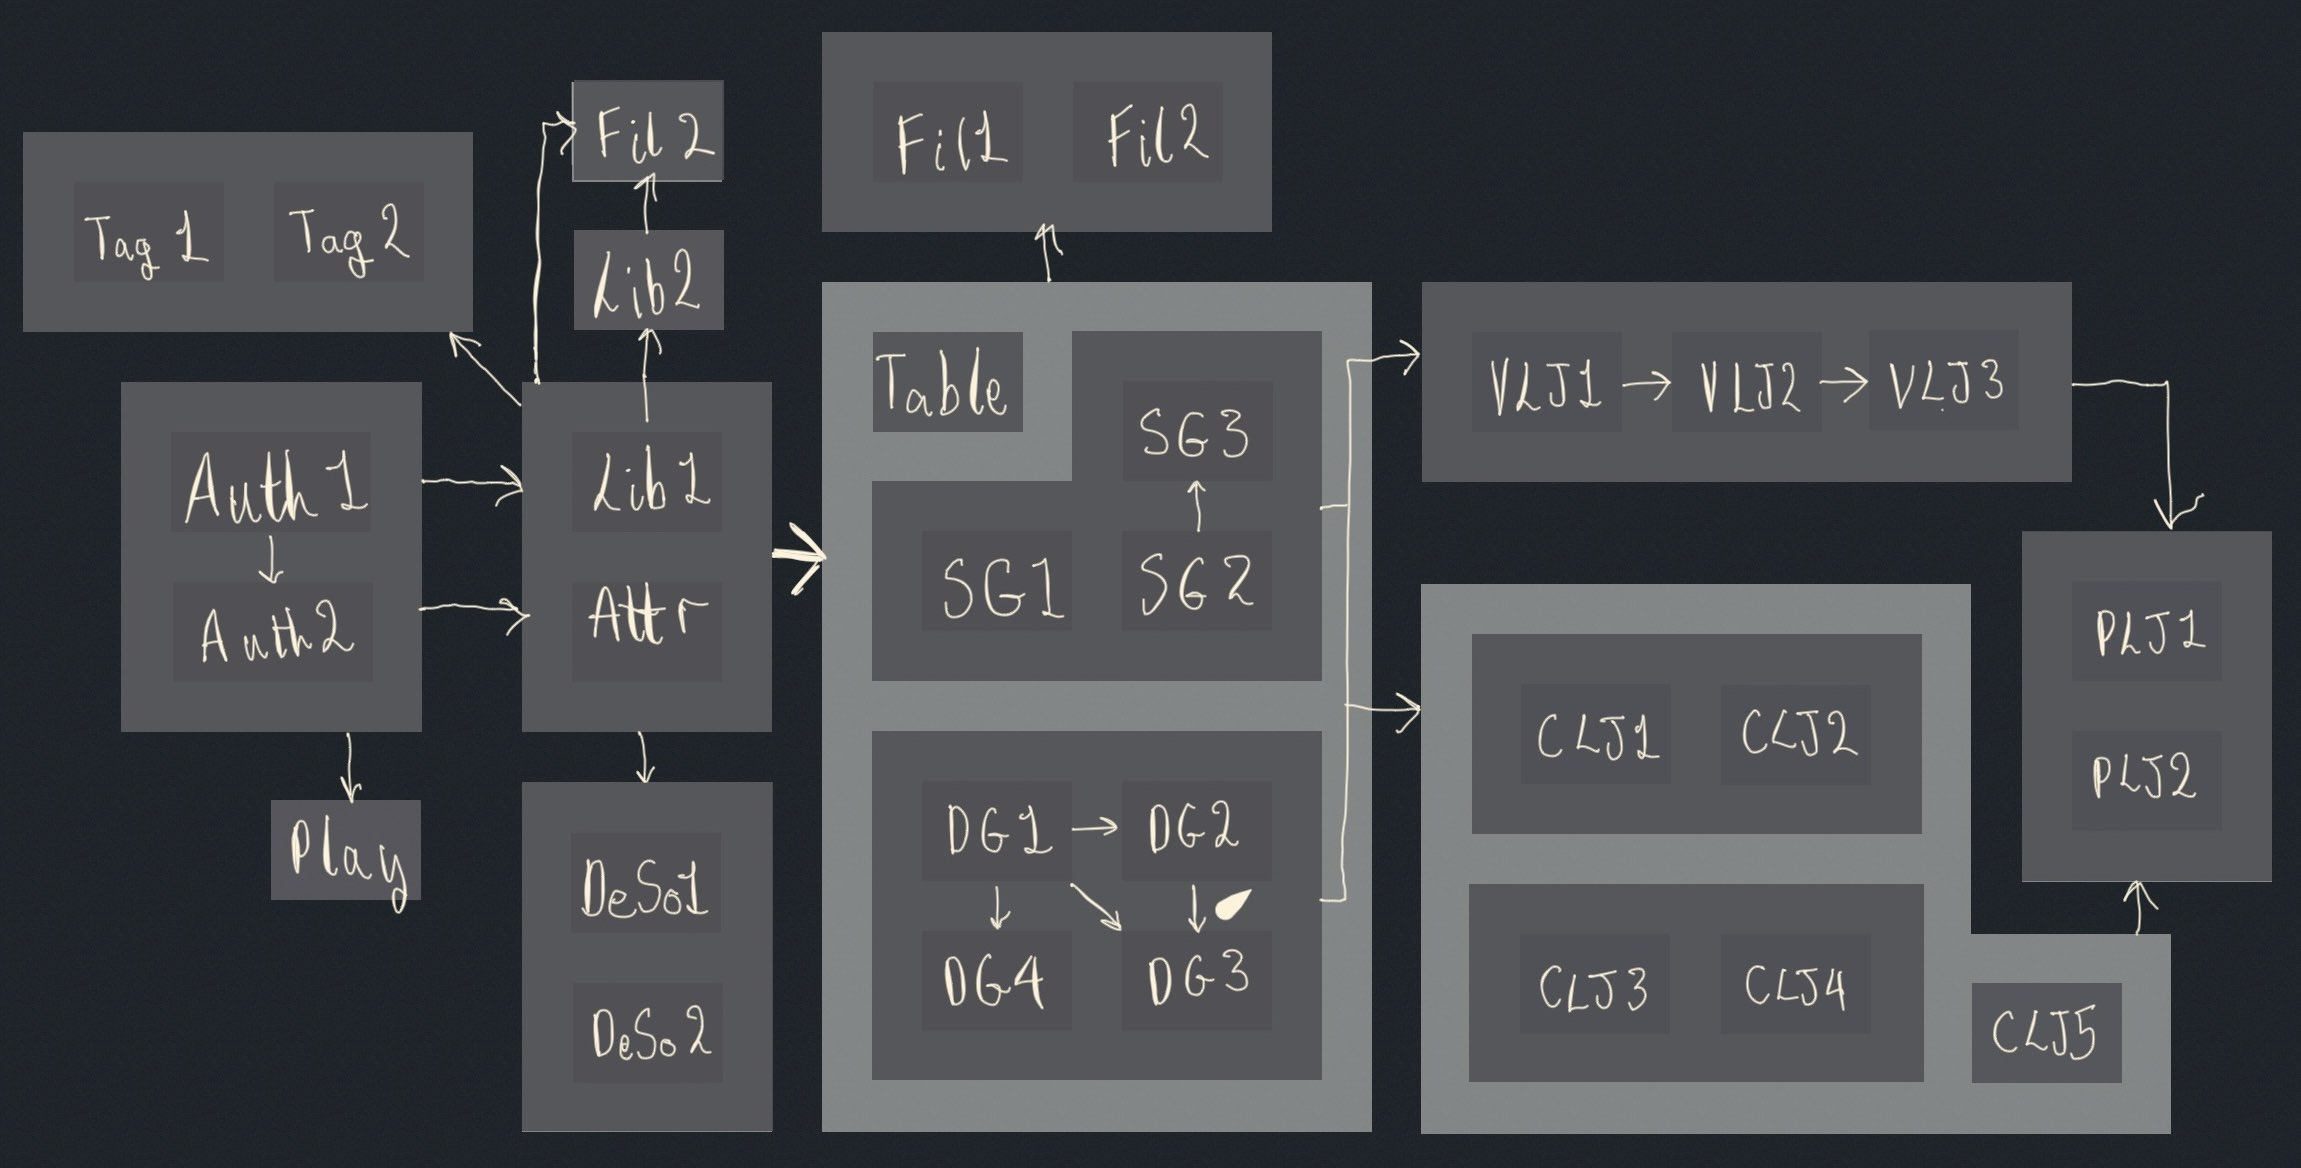
\includegraphics[scale=0.204]{Activity_Network_Diagram.jpg}
    \caption{Activity Network Diagram of Functional Dependencies}
\end{figure}

% User stories have been cut as it was deemed that their content overlapped too much with the functional requirements and as such were easy to cut to fit within the word limit

\section{Static Cartesian Graphs}
As can be seen in figure \ref{figure::ui::static_cartesian_graph} the coordinates for the songs directly map to the values for the metric for the axis. Clicking on a song will then render a line to the axis to show the exact value on the axis.
\begin{figure}
    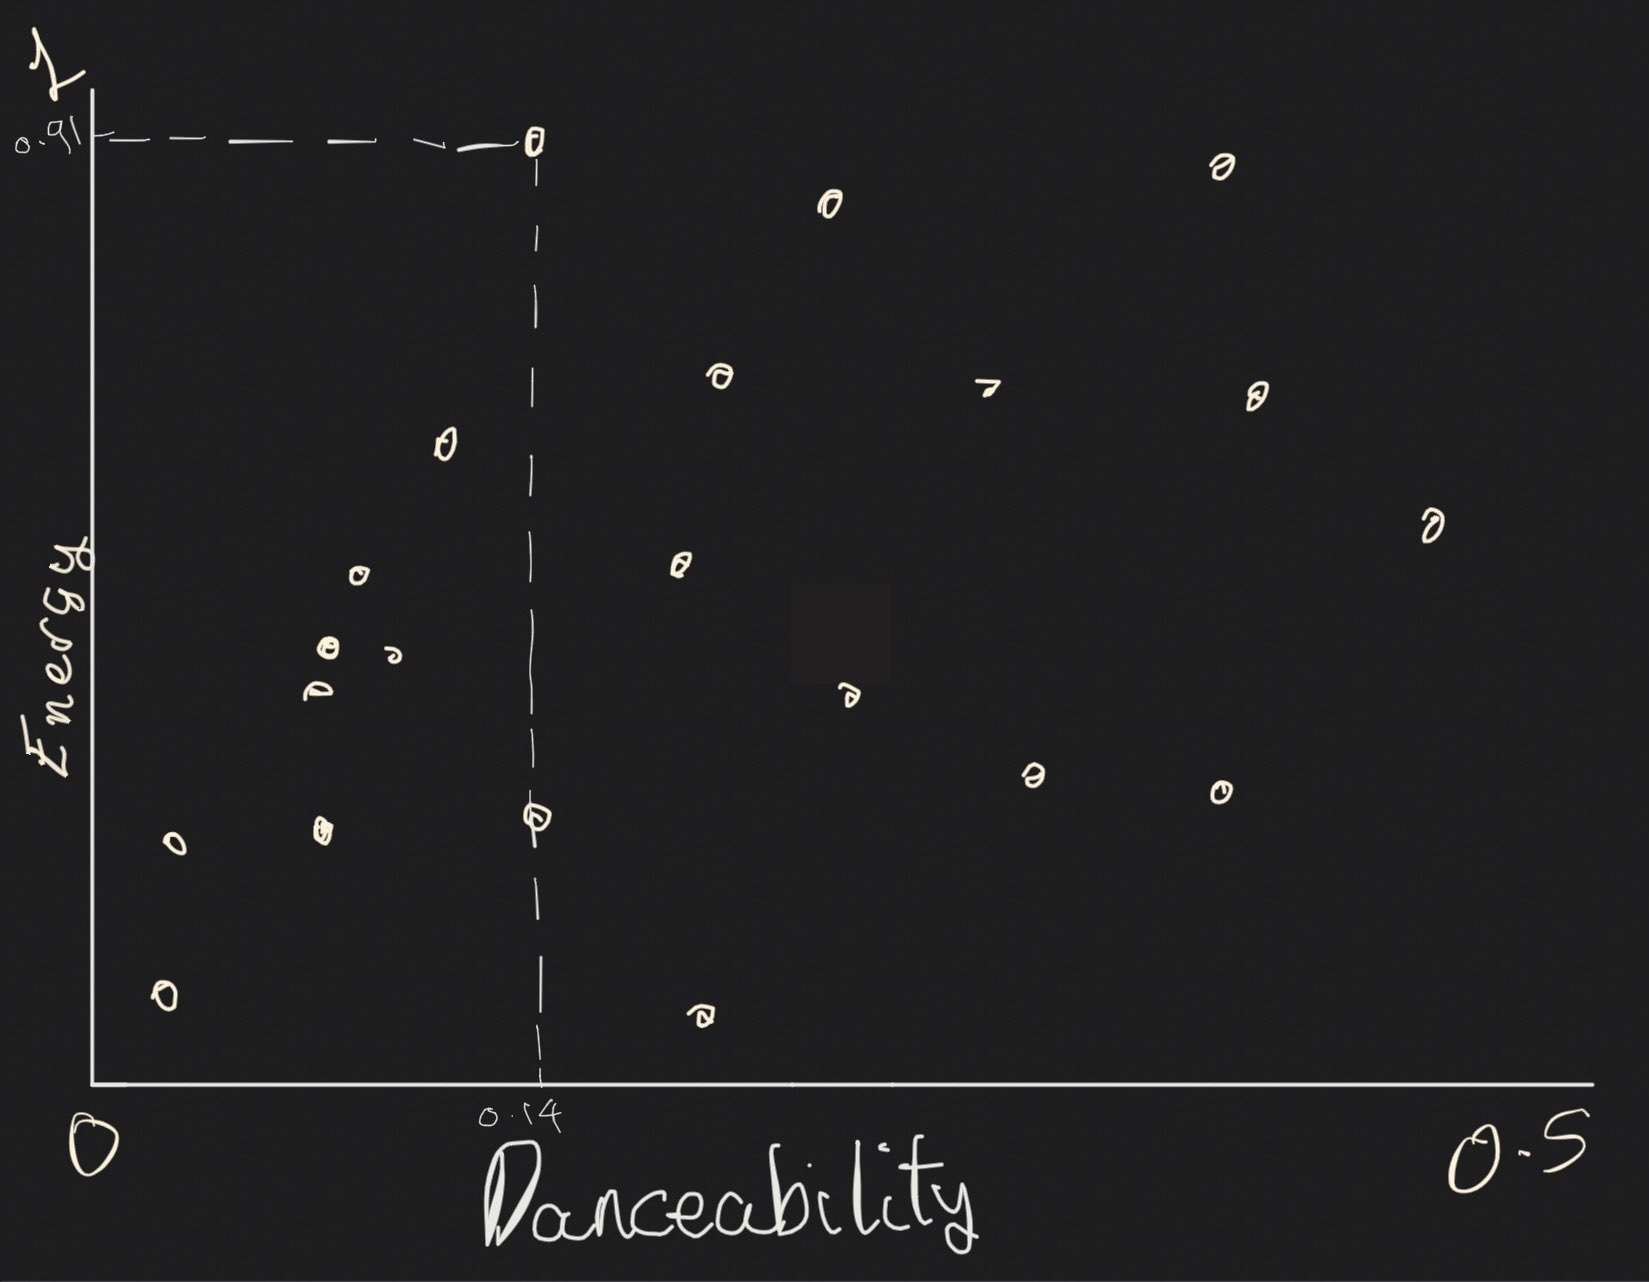
\includegraphics[angle=0, scale=0.251]{UI_Static_Cartesian_Graphs.jpg}
    \caption{Static Cartesian Graphs UI Mockup}
    \label{figure::ui::static_cartesian_graph}
\end{figure}

\section{Dynamic Similarity Graph}
\subsection{Building the Logical Dynamic Graph}
\subsubsection{Discrete Metrics} For each discrete metric in tables \ref{table::attributes} and \ref{table::metadata} a query is made. All songs that have the same value for this metric have the relationship component \texttt{SameMetric(100)} added to each other (\texttt{Metric} is replaced by the metric that has been queried, such as key or album). A weight of 100 is added to make it easier to interact with the continuous edges mentioned below.

\subsubsection{Continuous Metrics} Each continuous metric is queried for. Then for each song, all other songs are looped through performing the following:\begin{itemize}
    \item given song \texttt{A} and song \texttt{B}, find the difference between their values for the current continuous metric,
    \item divide this difference by the maximum possible difference for the current continuous metric to get a percentage similarity
    \item add a relation component, such as \texttt{A} --SimilarAcousticness(57.4\%)--\> \texttt{B} (the weight is the similarity percentage)
\end{itemize}

\subsection{Rendering the Dynamic Graph}
Firstly a song is selected at random. Then for each discrete relation component on this song, the target for the relation component is also rendered (along with the edge itself). Once all songs have been rendered with their discrete edges, each song adds its continuous edges to the graph.

Songs are pulled closer together depending on the strength of the weight for each edge. A weight of 100\% would pull the songs as close together as possible. If there are multiple weights between two songs then their overall similarity is used to decide how close they are to each other.

Each metric can be toggled to be inactive, meaning all edges for that metric are unrendered, with the song spheres moved to their new appropriate location based on the new overall weights of their edges.

\begin{figure}[h]
    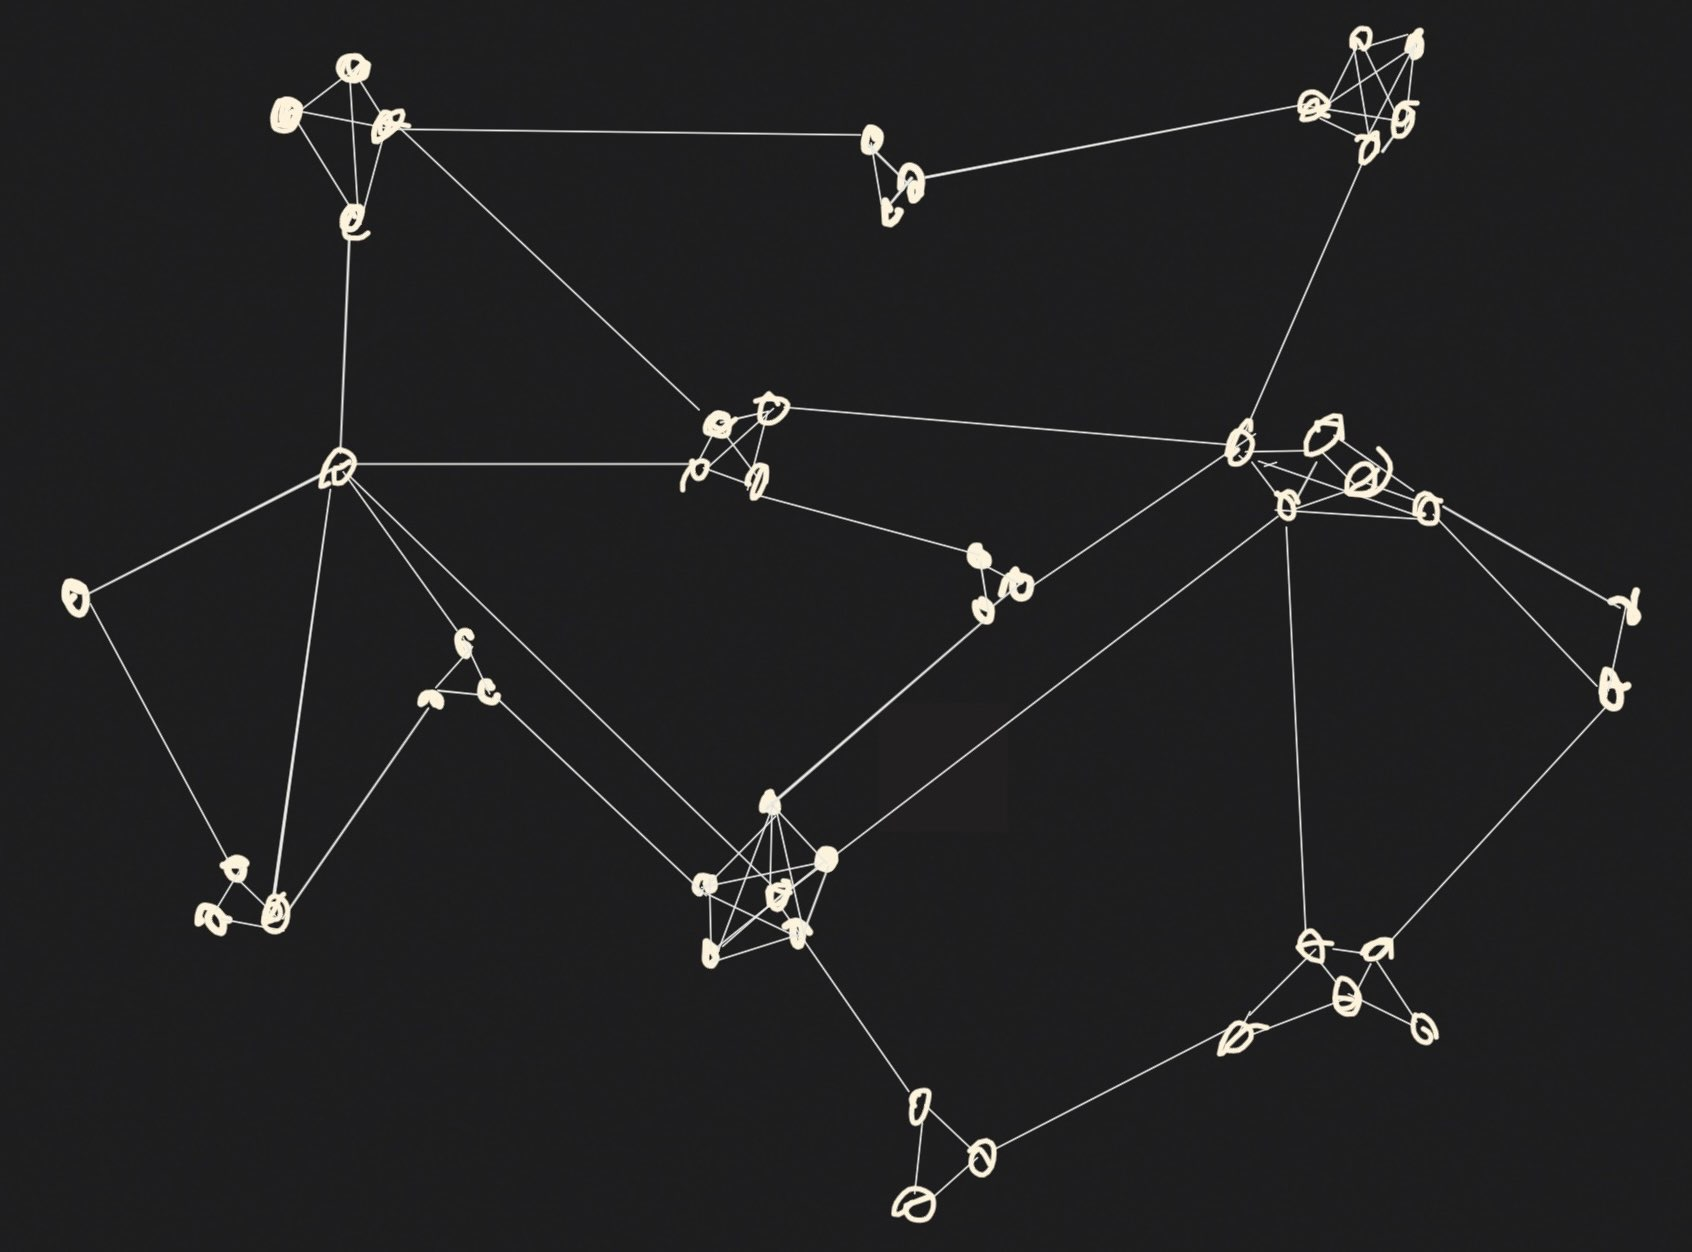
\includegraphics[angle=0, scale=0.251]{UI_Dynamic_Similarity_Graph.jpg}
    \caption{Dynamic Similarity Graph UI Mockup}
    \label{}
\end{figure}
\pagebreak

\section{Audio Journeys}
Audio journeys are simply the listening history, present and future for a user. These are normally shown in a list format but can also be shown as a directional line as shown in figure \ref{figure::ui::audio_journey_as_line}:\begin{itemize}
    \item Blue directional line: listening history of the user (limited either by number of songs or length of time)
    \item Blue song sphere: the current song being listened to
    \item Grey line: the upcoming songs in the queue
    \item Grey shaded region: subset of queue that will be played in a random order
\end{itemize}

\begin{figure}
    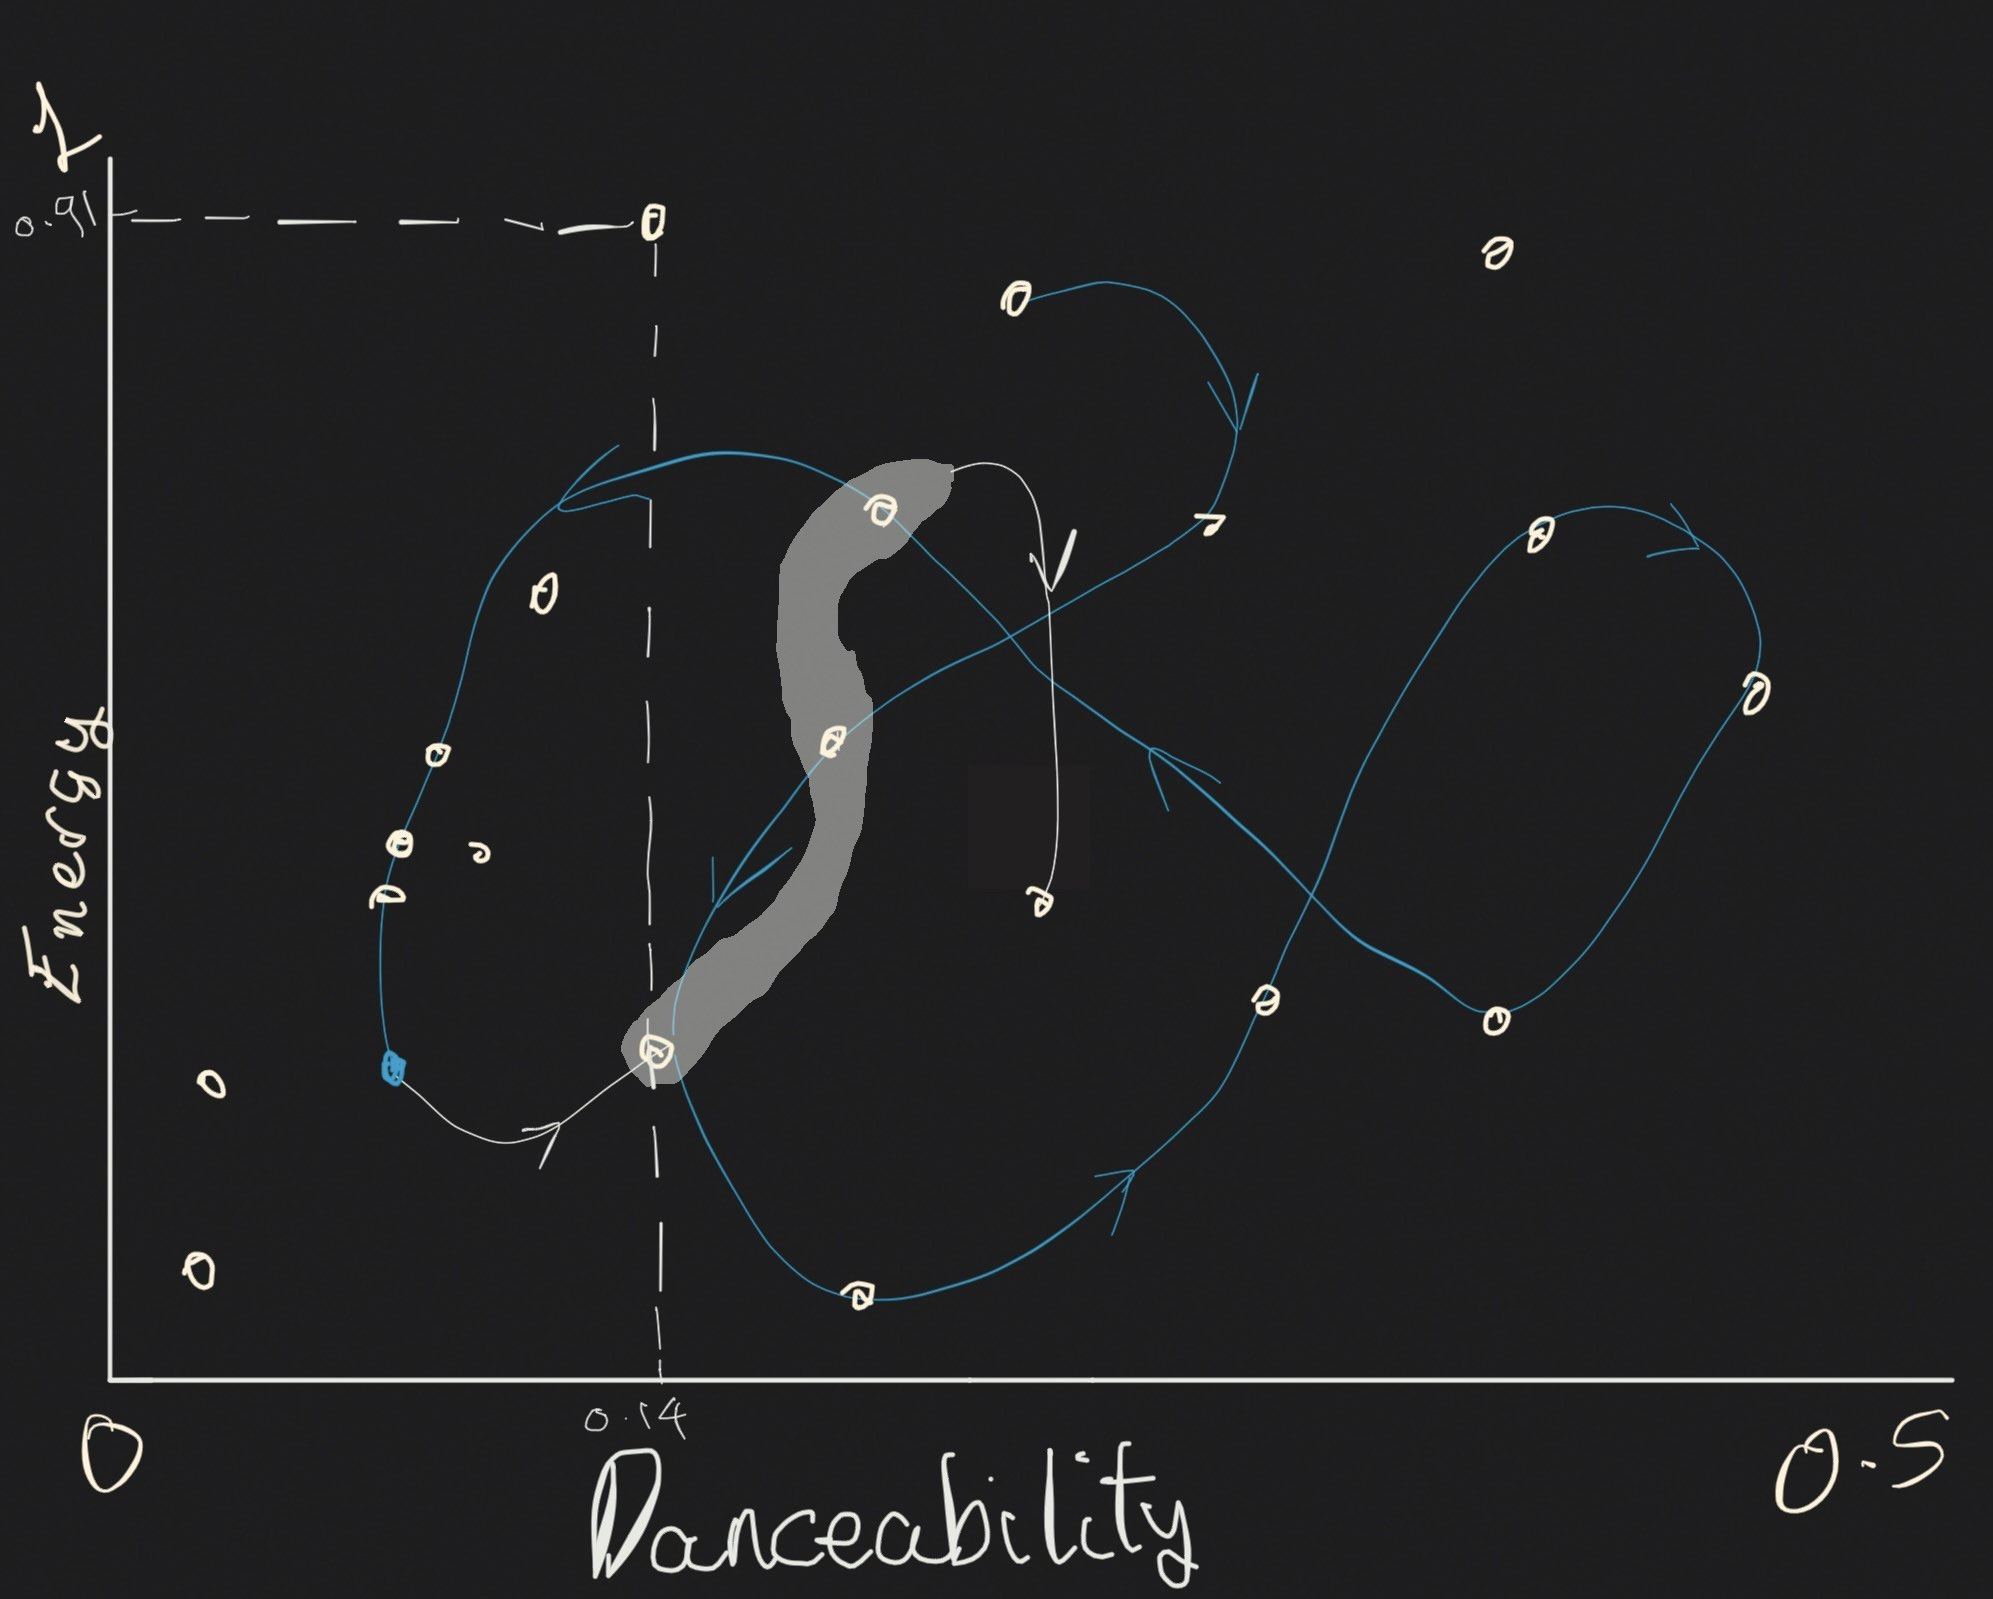
\includegraphics[angle=0, scale=0.1]{UI_Static_audio_journey.jpg}
    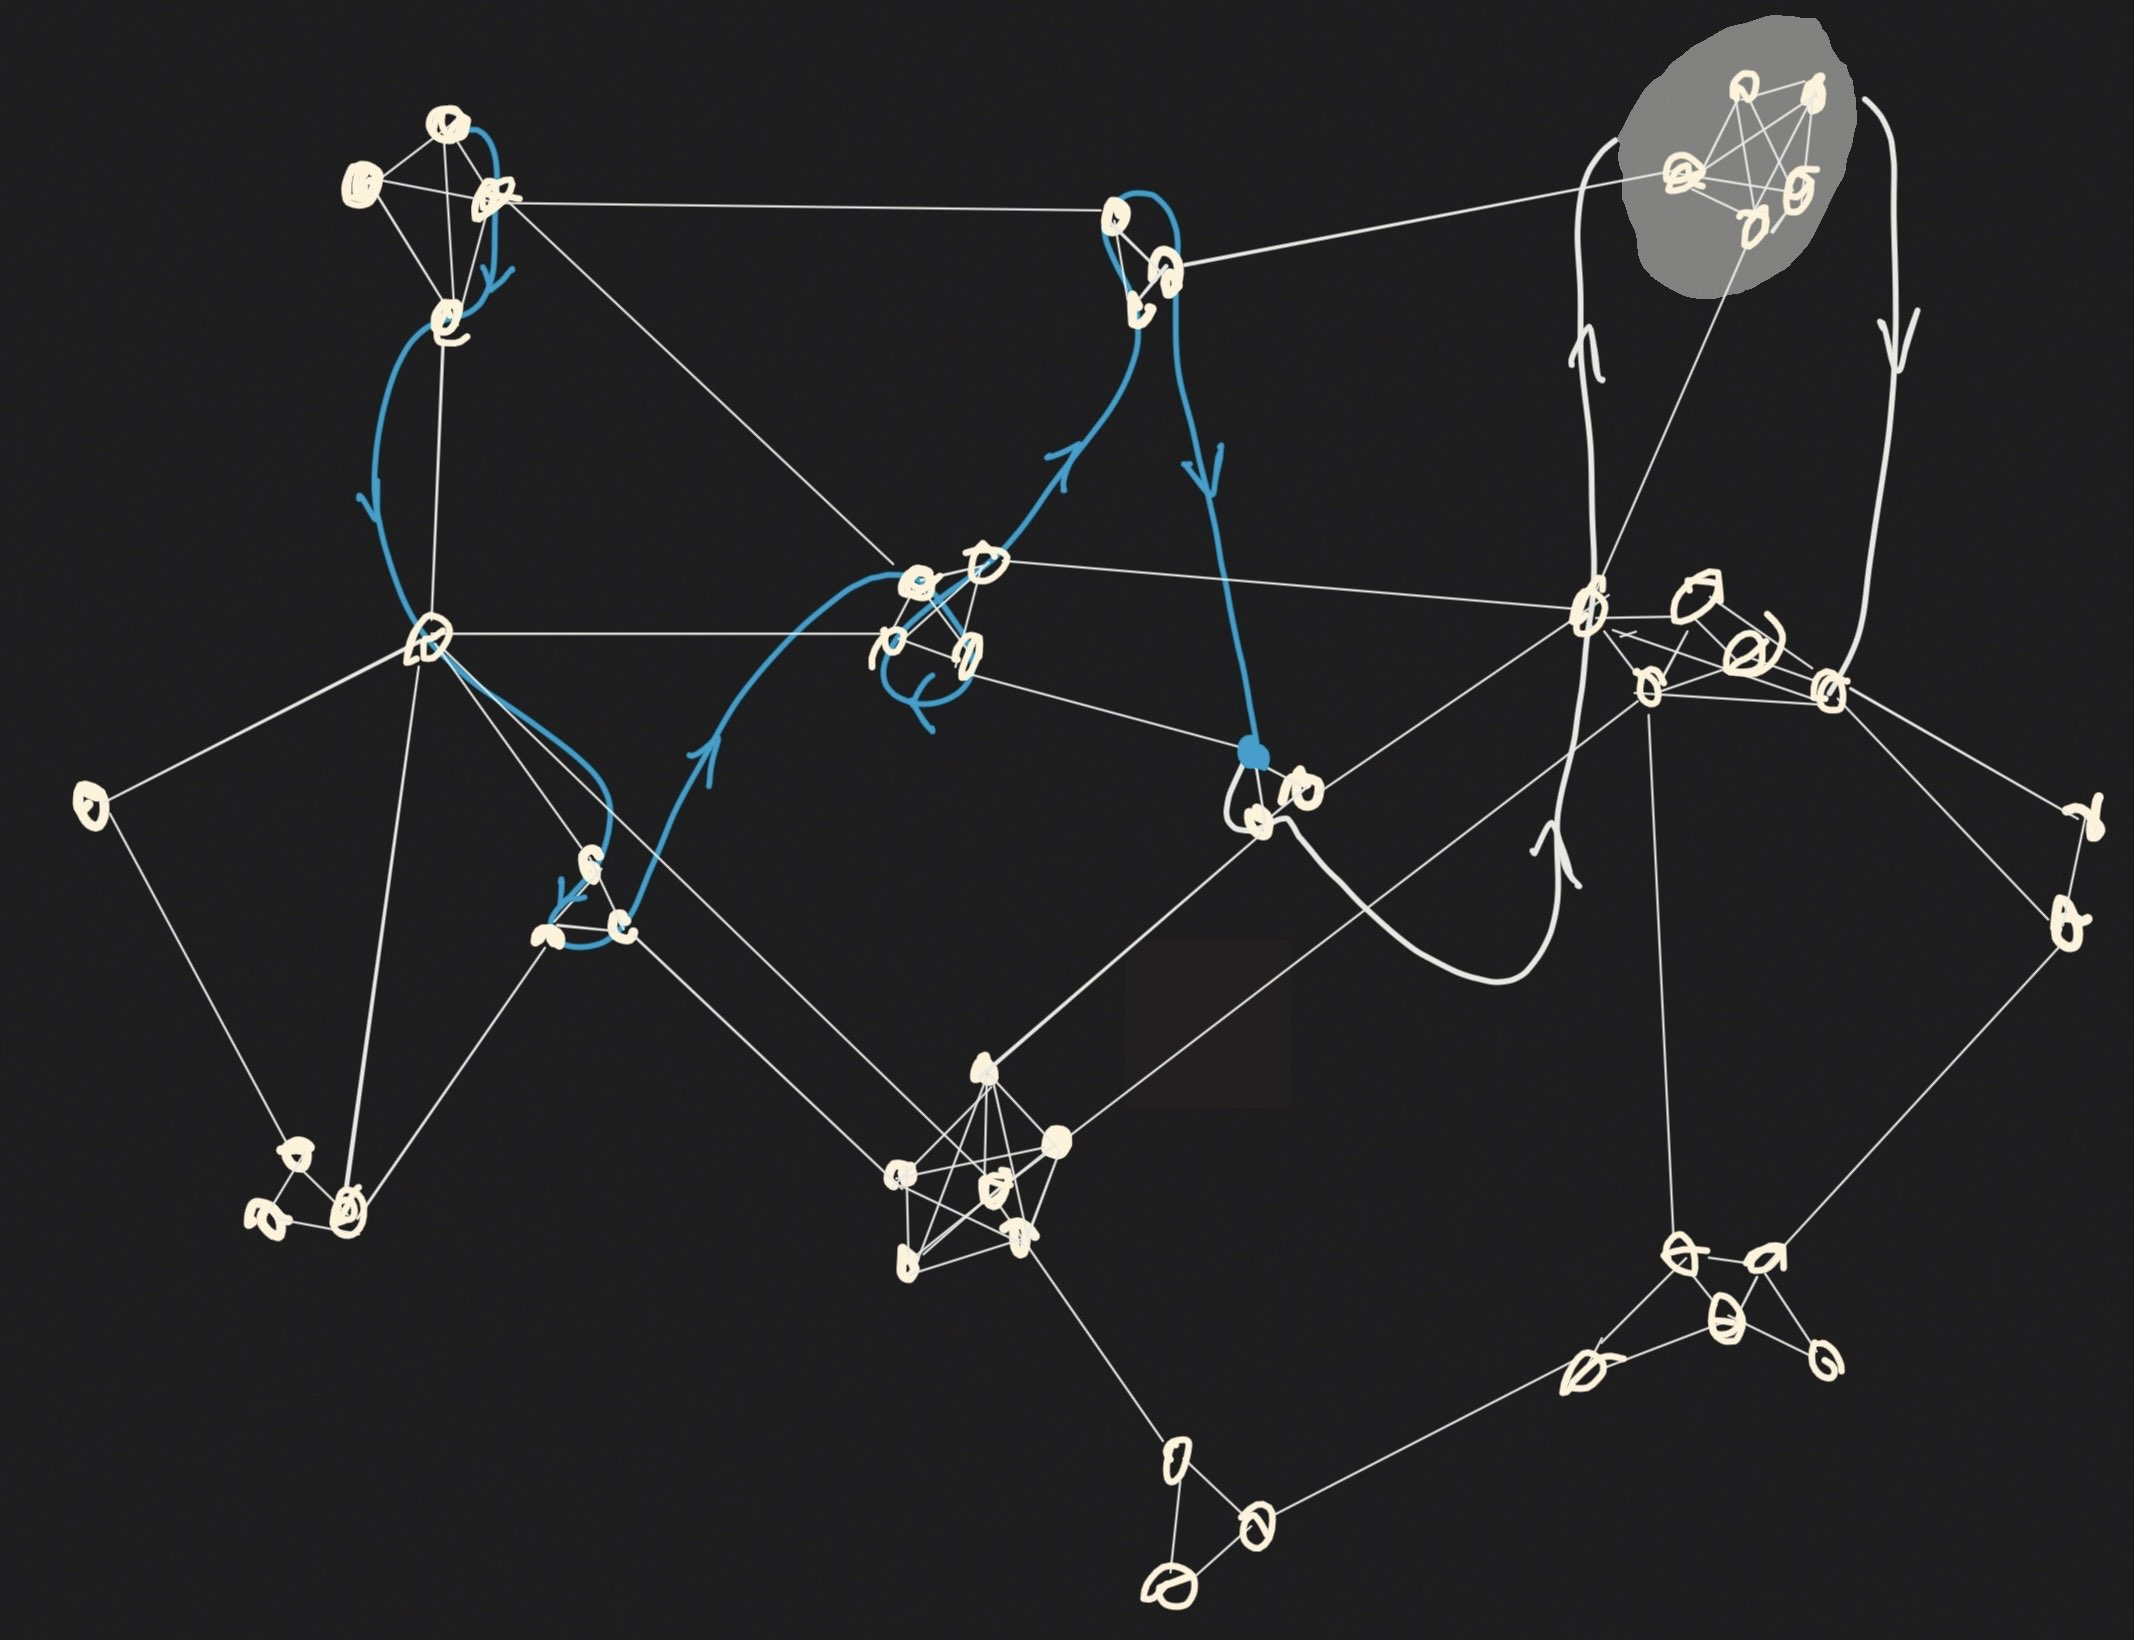
\includegraphics[angle=0, scale=0.1]{UI_Dynamic_audio_journey.jpg}
    \caption{Audio Journey on both Static and Dynamic Graph UI Mockup}
    \label{figure::ui::audio_journey_as_line}
\end{figure}

The upcoming line can also be moved by the user to easily go through different songs or clusters of songs. To listen to a subset of songs in a random order, they can be marked with a random region, where those songs will all be played, but in a random order that can be shuffled by the user. The line is more curved to help distinguish it from the pre-existing straight lines in the graphs.

%\section{TODO: Storyboards}%? How many do I have of these?